\documentclass[aip, jmp, amsmath, amssymb, reprint, floatfix]{revtex4-1}

\usepackage{graphicx}
\usepackage{dcolumn}
\usepackage{bm}
\usepackage{subfig}
\usepackage{afterpage}  
\usepackage{float}
\usepackage[font={footnotesize}]{caption}


\setlength{\parindent}{4em}
\setlength{\parskip}{0em}
\newcommand{\squeezeup}{\vspace{-4.5mm}}

\begin{document}

\title[Measurement of the Quenching Factor for Barium Fluoride Crystals]{Measurement of the Quenching Factor for Barium Fluoride Crystals}

\author{A. Hasse}
\affiliation{Department of High Energy Physics California Institute of Technology}

\author{D. Hitlin}
\affiliation{Department of High Energy Physics California Institute of Technology}


\date{\today}

\begin{abstract}
The energy of particles can be determined by measuring the scintillation light emitted by crystals such as barium fluoride. As the particles travel through the inorganic scintillator, Birk’s Law describes the amount of light emitted for a given energy lost. The ratio of dispersed energy is dependent on the mass of the particle; this is known as the quenching factor. Barium fluoride has two mechanisms of scintillation, a fast and a slow component, which are at different wavelengths, that determine how quickly photons are emitted. The ratios of energy from the fast and slow components from multiple photomultiplier tubes with varying quantum efficiency as a function of wavelength, determine the final quenching factor. We find that the quenching factors of the fast and slow components are substantially different.
We measure the response of the barium fluoride crystal fast and slow components to alpha particles of known energies coming from the decay of slight radium contamination in the crystals. Confirmation with the known values allows for analysis of energy readout from gamma, electron, and alpha particles. This data, along with the quenching factor, is valuable for many high-energy physics experiments in which inorganic scintillators are used to find the mass or energy of particles. We will also use the findings to study the physical mechanisms affecting the quenching factor.
\end{abstract}

\maketitle

\section{\label{sec:level1}Introduction}

Scintillation is light emitted by a material that absorbs deposited energy from particles. In the case of inorganic scintillators, electrons in crystals are excited from the valance band, the lowest energy state, to the conductance band or the exciton band. When electrons excite above ground state they leave a gap in the energy level. This gap, known as a hole, forms a pair with the electron and the couple traverses through the scintillator until an impurity in the crystal captures the instability. The impurities in scintillators have electronic levels amid the gap between the valence and exciton bands. Once the electron-hole pair is captured, the impurity de-excites by emitting scintillation. If the initial electron is elevated to the exciton band the resulting light is from the fast component. Conversely if the initial electron is elevated to the conductive band the resulting light is from the slow component. The electrons in the conductive band reach a phenomenon known as a metastable state, when the atomic system does not immediately decay to ground state, creating slower scintillation light resulting in the slow component \cite{scint}. 

The energy from scintillation light is measured using photodetectors. The amount of scintillation is linearly proportional to the energy deposited and the slope of the line correlates to particles' mass and energy. This relationship is used in high-energy particle physic experiments, like those at Fermi Lab, to detect and differentiate new particles. This system is referred to as the calorimeter and is made of crystals with adjacent photodetectors \cite{Mu2e}. 

Barium Fluoride ($BaF_2$) crystals, a type of inorganic scintillator, are of particular interest due to their exceptional fast component. For $BaF_2$ crystals the fast component is .6 nanoseconds (ns) and the slow component is 540 ns. $BaF_2$'s fast component emits light more quickly than any other scintillator of its kind \cite{BaF2specs}. A short decay mechanism provides more precision, measured as $\bm{\sqrt{\tau}}$ where $\bm{\tau}$ is the scintillation time, and allows for close successive events to be detected. In order to benefit from the short decay time the light from the fast component must be separated from the slow component. This relationship can be described by the non-linear energy loss through the lattice, known as Birk's constant or the quenching factor ($\bm{\alpha_Q}$). 

Birk's Law describes how light is lost as a function of energy lost  

\begin{eqnarray}
\ \bm{dL/dx = S * (dE/dx)/(1 + \alpha_Q * (dE/dx))}
\label{eq:one}.
\end{eqnarray}


where L is the amount of light detected, E is the energy of the particle, and S is a constant specific to the crystal \cite{BaF2scint}. The quenching factor is linearly dependent on energy and is different for the fast and slow component. We assume the relationship is in the form of 

\begin{eqnarray}
\ \bm{\alpha_Q = E_f * \alpha_f + E_s * \alpha_s}
\label{eq:two}.
\end{eqnarray}

where $\bm{E_f}$ and $\bm{E_s}$ are the proportions of fast and slow scintillation, respectively, and $\bm{\alpha_f}$ and $\bm{\alpha_s}$ are the quenching factors for the fast and slow component. $\bm{\alpha_Q}$ is found for a specific sensor and energy deposition and $\bm{E_f + E_s = 1}$ is determined from the convolution of the Barium Fluoride Emission spectrum and the quantum efficiency (QE)of the photodetector. Birk's constant is affected non-linearly by the mass and linearly by the energy of a particle. Despite scintillators' supposed linear relationship between energy deposited and light emitted, as particles increase in mass the quenching factor increases. 

The quenching factors for the fast and slow components are determined as a function of deposition energy using at least two photosensors. The expected linearity, calibration factor ($\bm{1/Q_e}$), can be determined using low mass decays such as gamma or electron sources with known kilo-electron-volt (keV) values ($\bm{RE_k}$). The calibration is the slope of known energy versus the measured energy from the sensor ($\bm{RE_m}$). Birk's constant, as a function of deposited energy, is determined from the measured scintillation of heavier particles, which are affected by non-linear energy loss, as a quotient of the known energy and the expected energy after the calibration factor is applied. 

\begin{eqnarray}
\ \bm{\alpha_Q = RE_k / (RE_m * 1/Q_e)}
\label{eq:three}.
\end{eqnarray}

This is repeated for each sensor at each energy level and equation four is plotted $\bm{\alpha_f}$ versus $\bm{\alpha_s}$.  

\begin{eqnarray}
\ \bm{\alpha_Q = E_f * \alpha_f + E_s * \alpha_s}
\label{eq:four}.
\end{eqnarray}

for each detector. The point of best intersection represents the quenching factor for the slow and fast component. Replacing the $\bm{\alpha_f}$ with the total $\bm{\alpha_Q}$ in Birk's Law then determines the scintillation from the fast component at a given energy. 

In our research we determined Birk's constant for the fast and slow component of $BaF_2$ for alpha particles at energies 4.8, 5.5, 6.0, and 7.7 MeV. We found $\bm{\alpha_Q, E_f,}$ and $\bm{E_s}$ for three photosensors, in our case Photomultiplier Tubes (PMTs). $\bm{\alpha_Q}$ was determined with low mass particles from four radioactive sources and $\bm{E_f + E_s = 1}$ was determined from integrating under the curve of the QE and $BaF_2$ emission spectrum convolution. 

The collected data and the subsequent analysis yield equations 

\begin{eqnarray}
\ \bm{\alpha_s = -0.1398072 * RE_k\alpha + 4.13497323}
\label{eq:five},
\end{eqnarray}

\begin{eqnarray}
\ \bm{\alpha_f = -0.45007859 * RE_k\alpha + 11.23363402}
\label{eq:six}.
\end{eqnarray}

with errors of 

\begin{table}[h]
    \begin{tabular}{ | l | l | l | l | p{2cm} |}
    \hline
    Component & 4800 & 5500 & 6000 & 7700 \\ \hline

    Slow & 1.36287 & 1.31089 & 1.2333 & 1.10977\\ \hline  

    Fast & 0.0290772 & 0.0310162 & 0.0319127 & 0.0313639\\ \hline
    \hline
    \end{tabular}
  \caption{These values represent the errors on the measured quenching factors at each keV energy. The errors were found from the covariance matrix from finding the point of best intersection}
\end{table}


These functions can be used in future high-energy physic experiments to isolate the fast component in $BaF_2$ for more precise detection of particles. 


\section{\label{sec:level1}Method}

The following section describes the method for the two main processes of our research: data collection and analysis. Experimentally we find the center of each energy peak, from each source, for three PMTs. In the analysis process we find the calibration factors and the quenching factors using our measurements and manufacturer specifications. 

\subsection{\label{sec:level2}Laboratory Equipment and Configuration}

The final experiment used three Photomultiplier Tubes; ultraviolet extended full spectrum, solarblind, and ultraviolet extended full spectrum with a shortpass filter. For both PMTs and the filter the manufacturer has provided the light intensity as a function of photon wavelength. We also used five radioactive sources. Four of the sources were low mass decays, electron or gamma; AmericiumBeryllium 241 (AmBe 241), Cesium 137 (Cs 137), Cobalt 60 (Co 60), and Sodium 22 (Na 22). Na 22 and Co 60 have particle decays at two keV values, which provided six points for calibration Table \ref{table:knownvalues}. The fifth source is alpha decay from natural Radium 226 impurities in the $BaF_2$ crystal, which decay at four energies \cite{Ra226}. The crystal used in each experiment remained the same. It had previously been found to have a relatively high concentration of impurities allowing for a higher rate of decay. 


\begin{table}[h]
    \begin{tabular}{ | l | l | p{2cm} |}
    \hline
    Source & AmBe 241 & Cs 137 \\ \hline

    Energy in keV & 59 & 662 \\ \hline  

    Source & Co 60 First Peak & Co 60 Second Peak  \\ \hline

    Energy in keV & 1170 & 1330 \\ \hline

    Source & Na 22 First Peak & Na 22 Second Peak \\ \hline

    Energy in keV & 511 & 1274 \\ \hline

    Source & Ra 226 First Peak & Ra 226 Second Peak \\ \hline

    Energy in keV & 4800 & 5500 \\ \hline

    Source & Ra 226 Third Peak & Ra 226 Fourth Peak \\ \hline

    Energy in keV & 6000 & 7700 \\ \hline
    \hline
    \end{tabular}
  \caption{These values are the previously known energy values of the particles from each radioactive source}
  \label{table:knownvalues}
\end{table}


In addition to our variables we used several pieces of equipment. The data compiler, caen, provides a clear user interface and was designed for physics problems of this kind \cite{caen}. A voltage box operating up to 5000 volts supplied the power for the PMTs. We also used an arduino circuit board and two A2302 temperature probes to collect the temperature in the laboratory while tests were active. Lastly the PMT, crystal, and source were in a light sealed box with cable panels to connect equipment inside and outside Figure \ref{fig:schem}. 

\begin{figure}
  \centering
    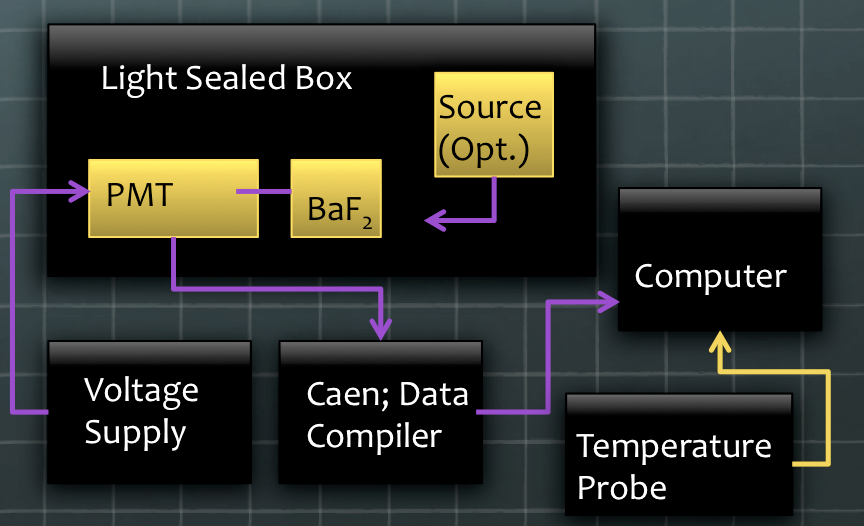
\includegraphics[width=.8\columnwidth]{schem.png}
  \caption{Equipment schematic; remained the same for every expeirmental trial in this research}
  \label{fig:schem}
\end{figure} 


\subsection{\label{sec:level2}Experimental Procedure}

Before recording any sources, the PMT must be supplied the desired voltage for 12 hours. As the PMT warms up the quantum efficiency is altered and after due time, 12 hours in our case, the PMT's temperature stabilizes. The arduino probe's temperature record was also launched to ensure the PMT was not affected from external heat fluctuations. 

For a given PMT the voltage and settings on the caen data compiler remain the same. Depending on the quantum efficiency of the PMT we set the voltage to maximize the gain and minimize background noise \cite{PMT}. The threshold, bin size, and gate length were also set. Raising the threshold diminishes background noise, but can also diminish noise from the source. The bin size sets a relative scale for the energy counts and takes into account the dispersion of source peaks so the highest source is not above the recorded channel. The gate length is in ns and regulates the amount of light detected for each collection point; it can also be used to lower the portion of the slow component seen \cite{caen}. 

\subsubsection{\label{sec:level3}Evaluating a PMT}

To begin collection with a PMT the lens and crystal are both decontaminated. The crystal is then wrapped on five of the faces with a shielding material to channel all of the scintillation into the PMT. The open face of the crystal is secured onto the PMT with grease and then the PMT and crystal are placed in the light sealed box and connected with coaxial cables to the voltage supply and caen. After the PMT has been left on for at least 12 hours the sources can be evaluated. Following standard radiation safety procedure we then place a source in the light sealed box within a couple inches of the crystal to increase interactions. Once the parameters are adequately set, the energy histogram is recorded. When the caen has enough counts in each bin to show an energy peak in the histogram with the desired resolution, data is saved, and we repeat the process with the three other sources and then the crystal alone for Ra 226. 

Each source varies in rate of decay and each PMT varies in the amount of light it can detect. Tests varied widely in recording length due to variations in QE and rate of decay. In order to complete a trial the energy peaks had to be visible above the background noise and have a reasonable resolution. The initial histogram shows the number of counts at each energy level. In the data analysis each energy peak will be isolated and the position recorded as the channel value for that specific set-up Figure \ref{fig:exhist}. 

\begin{figure}
  \centering
    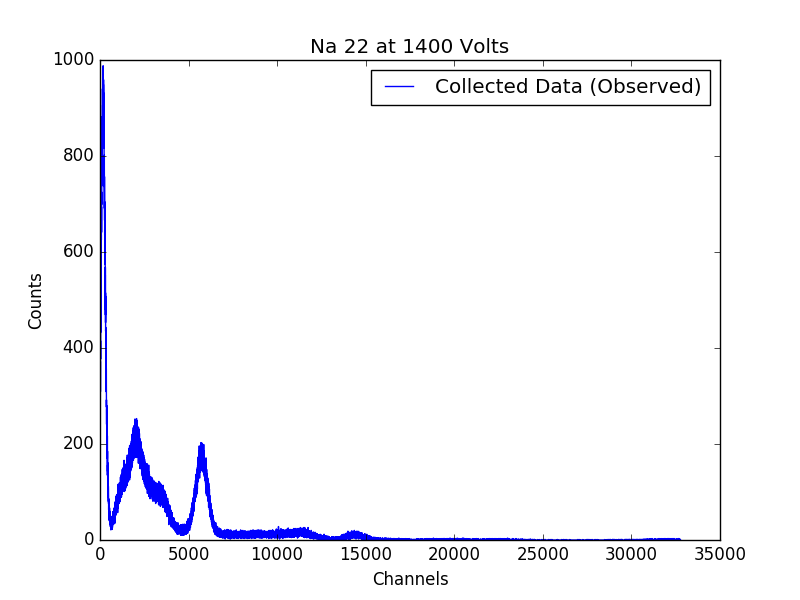
\includegraphics[width=.8\columnwidth]{na.png}
  \caption{Example of caen energy histogram; Na 22 Solarblind PMT}
  \label{fig:exhist}
\end{figure} 


\subsection{\label{sec:level2}Data Analysis}

Before beginning data collection we created unique python scripts to analyze our anticipated data. The first program extracts the histogram for each source from a text file and fits the energy peaks with a Gaussian. The Gaussian fit produces the central peak location in channels for each energy level. Then the known decay values for each source are used to find the conversion from channels to keV. The calibration factor is the slope of the line of best fit between each point. The conversion for each Ra 226 peak produces the expected keV value from channels using equation (9).

\begin{eqnarray}
\ \bm{RE_k = RE_m * (1/Q_e)}
\label{eq:nine}.
\end{eqnarray}

This is then compared to the known Ra 226 decays in keV to find the quenching factor. We repeated this process for each PMT and recorded the quenching factors as in equation (3). 

The second program is also repeated for each PMT. The script convolves the QE specifications from each PMT manufacturer and the emission spectrum for Barium Fluoride, which produces a four Gaussian representation of the fast and slow component proportions. The proportion of the area from each component produces $\bm{E_s, E_f}$. 

Lastly a final script requires the input of the quenching factor and PMT with $BaF_2$ convolutions as global lists. The subsequent functions then produce four energy plots of equation (2), where $\bm{\alpha_Q}$ uses data from each PMT. The closest intersection of the line represents ($\bm{\alpha_s, \alpha_f}$), the final quenching factors. To find these points we created a Mathematica script and solved the minimized cost function analytically. From this process the covariance matrix can be formed to determine the errors on each value. The four ($\bm{\alpha_s, \alpha_f}$), and their respective ($\bm{\sigma_s, \sigma_f}$) are then imported back to the python script to plot each fast and slow value against the corresponding energies for the final quenching factors. 

\section{\label{sec:level1}Results}

We determined $\bm{\alpha_Q, E_f,}$ and $\bm{E_s}$ for each PMT. $\bm{\alpha_f}$ and $\bm{\alpha_s}$ at the four Ra 226 energy peak values, 4.8, 5.5, 6.0, and 7.7 MeV. The fast and slow proportion was also found for each PMT. For each PMT we fit every source with a Gaussian function which yielded the following parameter fits Figure \ref{fig:gaussfits}. Missing data is from trials that did not produce resolved energy peaks to fit a Gaussian. Each PMT still has enough peak values to complete the analysis. 

\begin{figure}
  \centering
    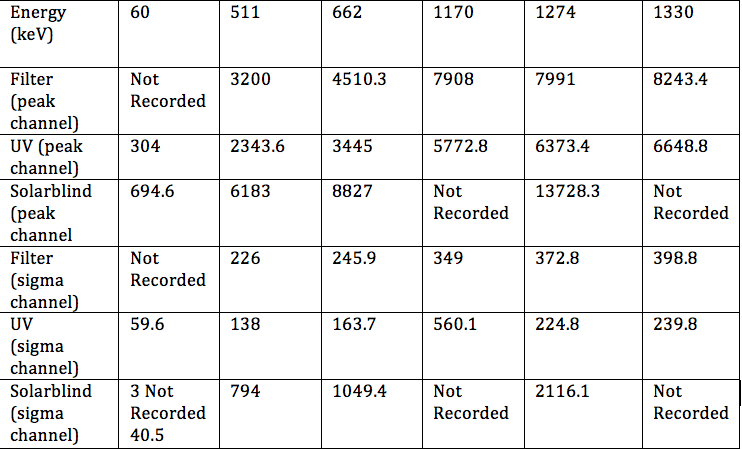
\includegraphics[width=.9\columnwidth]{gaussfits.png}
  \caption{Table with the recorded gaussian fit parameters from all experiments}
  \label{fig:gaussfits}
\end{figure} 

\noindent
Using the peak value and associated sigma, the keV to channels conversion Figure \ref{fig:chanf}, Figure \ref{fig:chanuv}, and Figure \ref{fig:chansb} was determined for each PMT; 

\begin{table}
    \begin{tabular}{ | l | l | p{2cm} |}
    \hline
    PMT & Channels to keV\\ \hline

    UV with filter & 6.33012509\\ \hline  

    UV & 4.984\\ \hline

    Solarblind & 12.0694256\\ \hline
    \hline
    \end{tabular}
    \caption{These values represent the slope of the line from channels (found from the caen output) to keV (from the known values) for each PMT.}
    \label{table:chan_kev}
\end{table}

\begin{figure}[h]
  \centering
    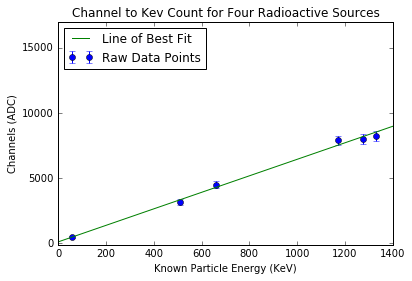
\includegraphics[width=.8\columnwidth]{chanf.png}
  \caption{UV with filter Calibration Function}
  \label{fig:chanf}
\end{figure} 

\begin{figure}[h]
  \centering
    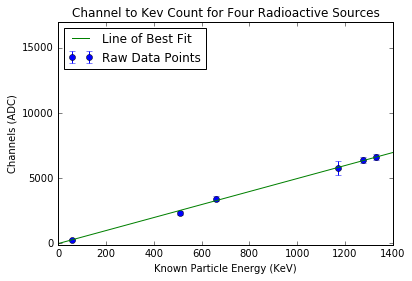
\includegraphics[width=.8\columnwidth]{chanuv.png}
  \caption{UV Calibration Function}
  \label{fig:chanuv}
\end{figure} 

\begin{figure}[h]
  \centering
    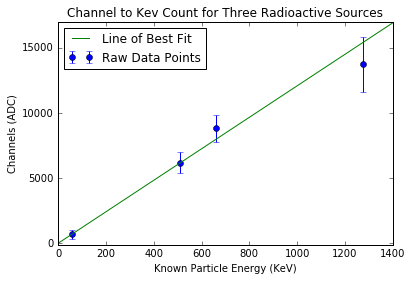
\includegraphics[width=.8\columnwidth]{chansb.png}
  \caption{Solarblind Calibration Function}
  \label{fig:chansb}
\end{figure} 


The inverse slope of the best fit line multiplied by the Ra 226 peak channel values yielded the expected energy in keV, which then determined the quenching factors $\bm{\alpha_Q}$ Figure \ref{fig:qff}, Figure \ref{fig:qfuv}, and Figure \ref{fig:qfsb}.

The inverse slope of the best fit line multiplied by the Ra 226 peak channel values yielded the expected energy in keV, which then determined the quenching factors $\bm{\alpha_Q}$ Figure \ref{fig:qff}, Figure \ref{fig:qfuv}, and Figure \ref{fig:qfsb}.

\begin{table}
    \begin{tabular}{ | l | l | l | l | p{2cm} |}
    \hline
    PMT & 4800 & 5500 & 6000 & 7700\\ \hline

    UV with filter & 2.976 & 2.849 & 2.704 & 2.460\\ \hline  

    UV & 3.269 & 3.136 & 2.977 & 2.702\\ \hline

    Solarblind & 5.155 & 4.789 & 4.475 & 4.166\\ \hline
    \hline
    \end{tabular}
    \caption{These values represent the quenching factor found at each energy level for eahc PMT. These were determined by comparing the expected conversion keV value with the known keV value for each Ra 226 peak}
    \label{table:quench}
\end{table}

\begin{figure}
  \centering
    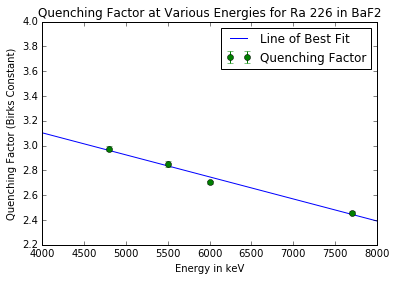
\includegraphics[width=.8\columnwidth]{qff.png}
  \caption{UV with filter Quenching Factors}
  \label{fig:qff}
\end{figure} 

\begin{figure}
  \centering
    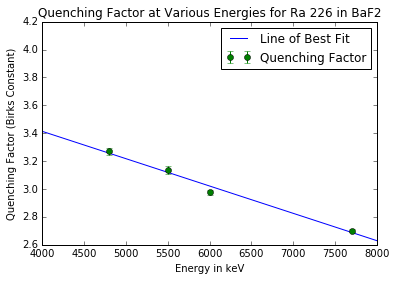
\includegraphics[width=.8\columnwidth]{qfuv.png}
  \caption{UV Quenching Factors}
  \label{fig:qfuv}
\end{figure} 

\begin{figure}
  \centering
    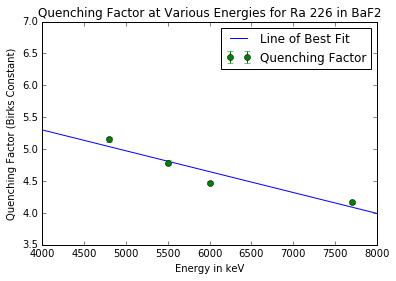
\includegraphics[width=.8\columnwidth]{qfsb.png}
  \caption{Solarblind Quenching Factors}
  \label{fig:qfsb}
\end{figure} 

The emission spectrum of Barium Fluoride was plotted and fitted with four Gaussians. Using this fit we convolved each QE spectrum Figure \ref{fig:FitsBaF2} to find $\bm{E_f}$ and $\bm{E_s}$ Figure \ref{fig:convf}, Figure \ref{fig:convuv}, and Figure \ref{fig:convsb}.

\begin{table}
    \begin{tabular}{ | l | l | p{2cm} |}
    \hline
    PMT & Fast Percentage & Slow Percentage\\ \hline

    UV with filter & 0.104 & 0.895\\ \hline  

    UV & 0.112 & 0.887\\ \hline

    Solarblind & 0.558 & 0.441\\ \hline
    \hline
    \end{tabular}
    \caption{These values represent the percentage of light that is from the fast and slow component for each PMT. They are defined as the area under the first two and last two Gaussians of the convolution of the $BaF_2$ emission spectrum and the QE of each PMT}
    \label{table:fastvsslow}
\end{table}

\begin{figure}
  \centering
    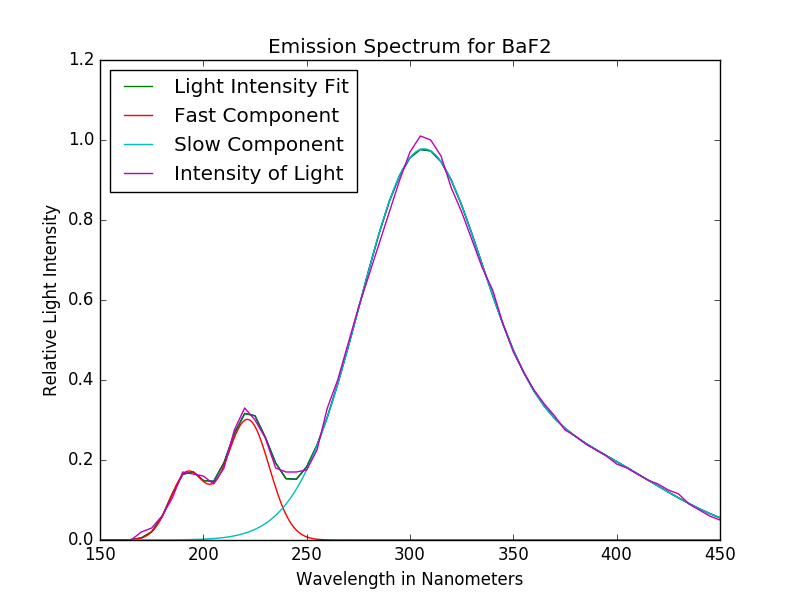
\includegraphics[width=.8\columnwidth]{FitsBaF2.png}
  \caption{Barium Fluoride emission spectrum}
  \label{fig:FitsBaF2}
\end{figure} 

\begin{figure}
  \centering
    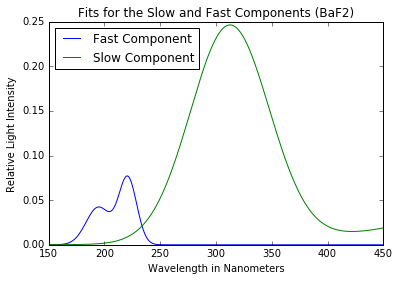
\includegraphics[width=.8\columnwidth]{convf.png}
  \caption{UV with filter Convolution}
  \label{fig:convf}
\end{figure} 

\begin{figure}
  \centering
    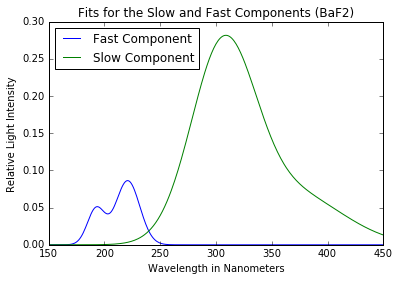
\includegraphics[width=.8\columnwidth]{convuv.png}
  \caption{UV Convolution}
  \label{fig:convuv}
\end{figure} 

\begin{figure}
  \centering
    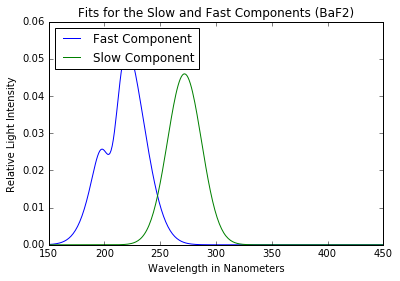
\includegraphics[width=.8\columnwidth]{convsb.png}
  \caption{Solarblind Convolution}
  \label{fig:convsb}
\end{figure} 

We plotted our determined values in this form for every Ra 226 peak, Figure 14, Figure 15, Figure 16, and Figure 17, with equation (2). Solving for the point of best intersection, (\bm{$\alpha_s, \alpha_f}$), at each energy level the quenching factor as a function of energy is shown in equations (10) and (11) with respective errors in equations (12) and (13). 

\begin{eqnarray}
\ bm{\alpha_s = -0.1398072 * RE_k\alpha + 4.13497323}
\label{eq:ten}
\end{eqnarray}

\begin{eqnarray}
\ bm{\alpha_f = -0.45007859 * RE_k\alpha + 11.23363402}
\label{eq:eleven}
\end{eqnarray}

\begin{table}
    \begin{tabular}{ | l | l | p{2cm} |}
    \hline
    Component Error & 4800 & 5500 & 6000 & 7700\\ \hline

    Slow Error & 1.362 & 1.310 & 1.233 & 1.109\\ \hline  

    Fast Error & 0.029 & 0.031 & 0.031 & 0.031\\ \hline
    \hline
    \end{tabular}
    \caption{These values represent the error on each fast and slow quenching factor determined from the covariance matrix in the calculation of the point of best intersection.}
    \label{table:fastvsslow}
\end{table}

\begin{figure}
  \centering
    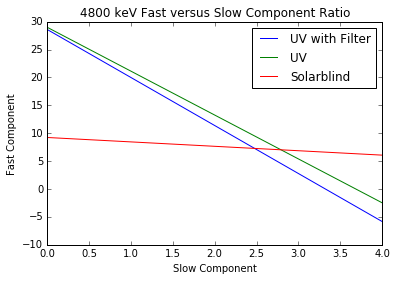
\includegraphics[width=.8\columnwidth]{first.png}
  \caption{Ra 226 4800 point of best intersction for the fast and slow component quenching factors}
  \label{fig:first}
\end{figure} 

\begin{figure}
  \centering
    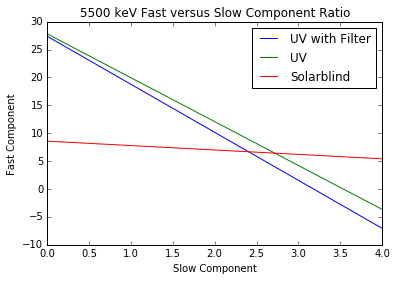
\includegraphics[width=.8\columnwidth]{second.png}
  \caption{Ra 226 5500 point of best intersction for the fast and slow component quenching factors}
  \label{fig:second}
\end{figure} 

\begin{figure}
  \centering
    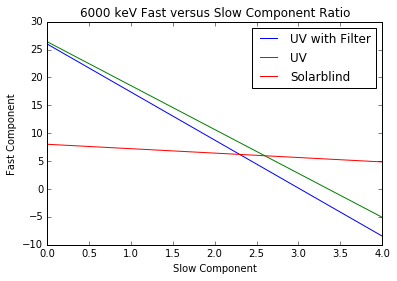
\includegraphics[width=.8\columnwidth]{third.png}
  \caption{Ra 226 6000 point of best intersction for the fast and slow component quenching factors}
  \label{fig:third}
\end{figure} 

\begin{figure}
  \centering
    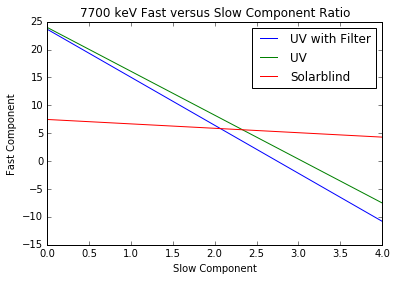
\includegraphics[width=.8\columnwidth]{fourth.png}
  \caption{Ra 226 7700 point of best intersction for the fast and slow component quenching factors}
  \label{fig:fourth}
\end{figure}
 

\noindent
Figure \ref{fig:qf} shows Birk's constant as a function of energy for the fast and slow component for alpha particle interactions with Barium Fluoride crystals.

\begin{figure}
  \centering
    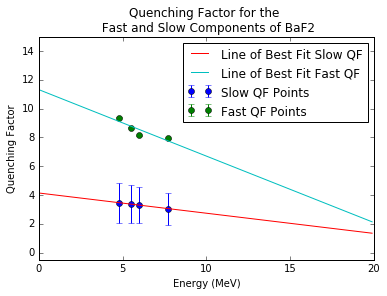
\includegraphics[width=.8\columnwidth]{qf.png}
  \caption{Final Quenching Factor Function}
  \label{fig:qf}
\end{figure} 


\section{\label{sec:level1}Discussion}


The separation of light from the fast and slow components for $BaF_2$ can be determined for any alpha particle from the measured slow and fast quenching factors. The total light from the fast component is found by solving Birk's Law, equation (1), to be a function of the integral of energy lost per distance (citation). 


The total energy is also determined using the above analysis. The integral of $\bm{dE/dx}$ is the total energy from the particle which is already known. By replacing general $\bm{\alpha_Q}$ with $\bm{\alpha_f}$ for the particles energy the light yield can be determined. 

In high energy physics experiments collaborators are trying to determine the energy or mass of a particle. Instead $\bm{dL/dx}$ is known from the calorimeter. For experiments of this nature, our measured Birk's constants will allow for precision in alpha particle discoveries using Barium Fluoride. 

\section{\label{sec:level1}Acknowledgements}
\squeezeup

The California Institute of Technology and its Student Faculty Programs office made the measurement of the quenching factor for barium fluoride crystals possible. A. Hasse would also like to express her deep gratitude towards Professor David Hitlin, Jake Kim, and Jason Trevor and the High Energy Physics group for this opportunity and their continuing support. 
\squeezeup

\section{\label{sec:level1}References}
\squeezeup

\begin{thebibliography}{9}
\bibitem{BaF2specs} 
Saint Gobain Ceramics and Plastics Inc. 
\textit{$BaF_2$ Barium Fluoride Scintillation Material}. 
2014.
 
\bibitem{Mu2e} 
Bartosvek, L., et. al.
\textit{Mu2e Technical Design Report}.
Fermi National Accelerator Laboratory. 
 
\bibitem{caen} 
CAEN SpA
\textit{Electronic Instrumentation DPSD Register Description}
\\\texttt{http://www-cs-faculty.stanford.edu/\~{}uno/abcde.html}
2013

\bibitem{scint} 
L'Annunziata, M.
\textit{Handbook of Radioactivity Analysis}.
2003

\bibitem{BaF2scint} 
Matulewicz, T.
\textit{Quenching of Scintillation in $BaF_2$ for Light Charged Particle}.
14021 Caen Cedex, France. 1967.

\bibitem{PMT} 
Hamamatsu
\textit{Photomultiplier Tubes, Basics, and Applications}.
2007

\bibitem{Ra226} 
Polischuk, O., Belli, P., Bernabei, R., Capella, F., Caracciolo, V., Cerulli, R., . . . Tretyak, V.
\textit{Radioactive contamination of BaF2 crystal scintillator}.
Nuclear Institute. 2009

\end{thebibliography}

\squeezeup

\section{\label{sec:level1}Appendix}


\begin{figure*}
  \centering
  \subfloat[\label{fig:2UVAmBefit} AmBe 241 UV PMT]{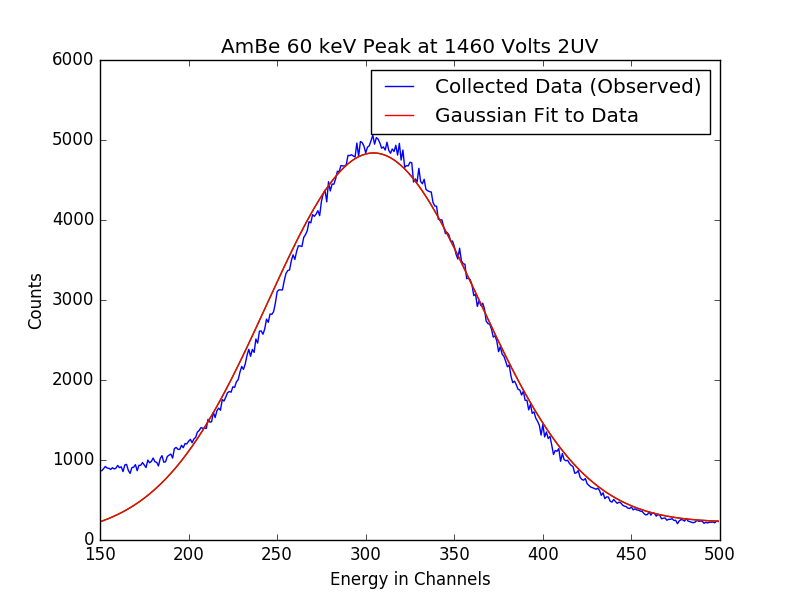
\includegraphics[width=.8\columnwidth]{2UVAmBefit.png}}%
  \qquad
  \subfloat[\label{fig:2UVCsfit} Cs 137 UV PMT]{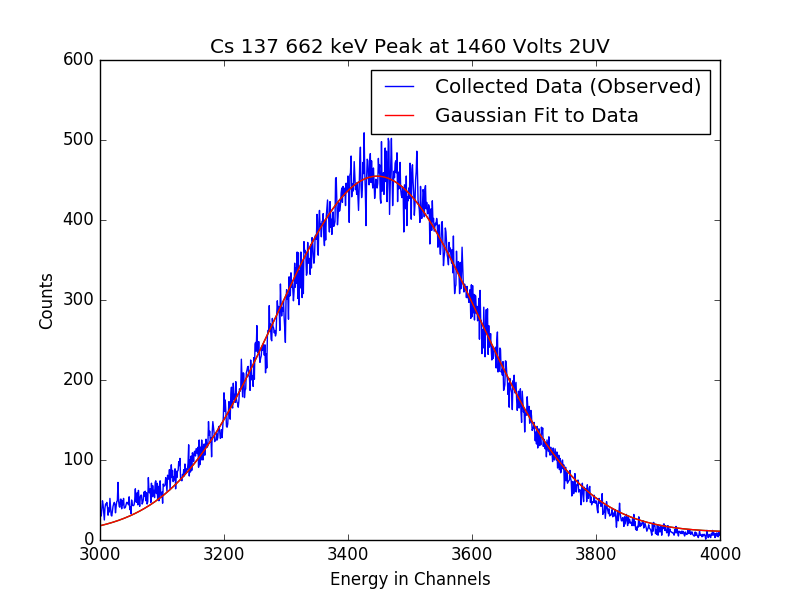
\includegraphics[width=.8\columnwidth]{2UVCsfit.png}}%
  \qquad
  \subfloat[\label{fig:2UVCo1fit} Co 60 Peak 1 UV PMT]{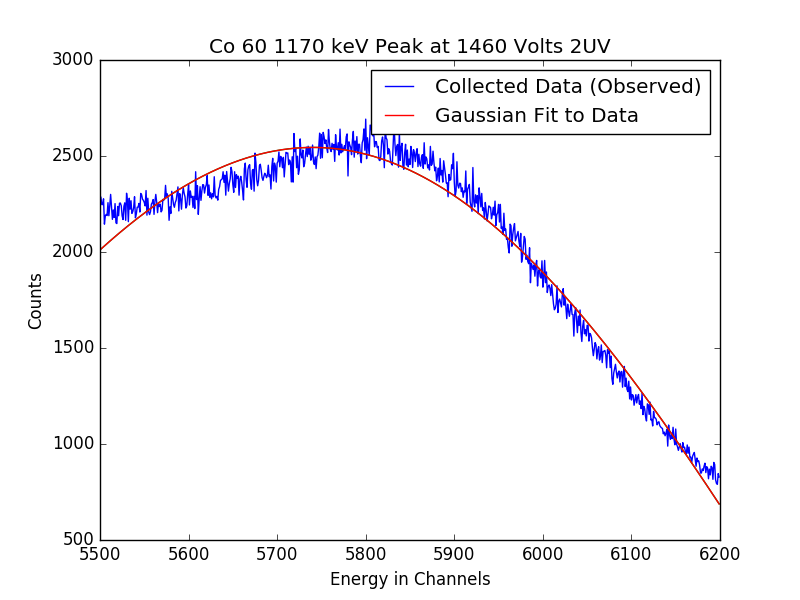
\includegraphics[width=.8\columnwidth]{2UVCo1fit.png}}%
  \qquad
  \subfloat[\label{fig:2UVCo2fit} Co 60 Peak 2 UV PMT]{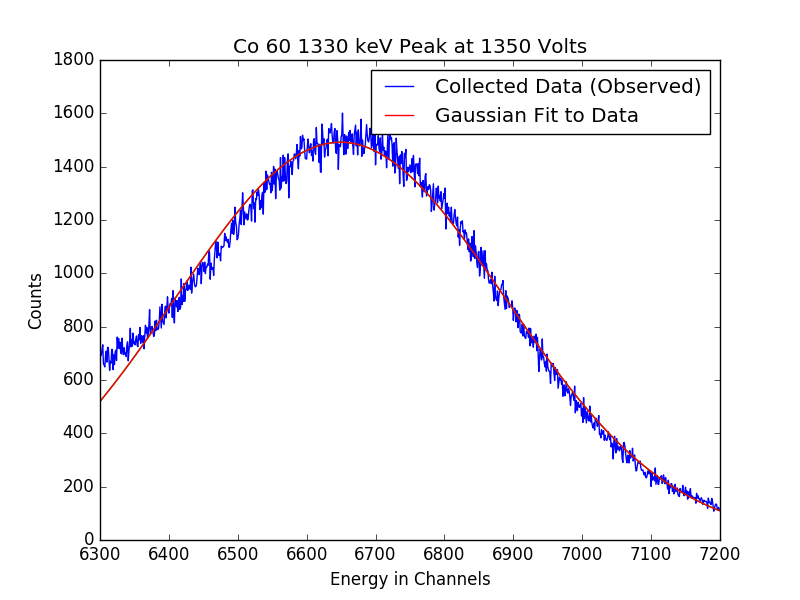
\includegraphics[width=.8\columnwidth]{2UVCo2fit.png}}%
  \qquad
  \subfloat[\label{fig:2UVNa1fit} Na 22 Peak 1 UV PMT]{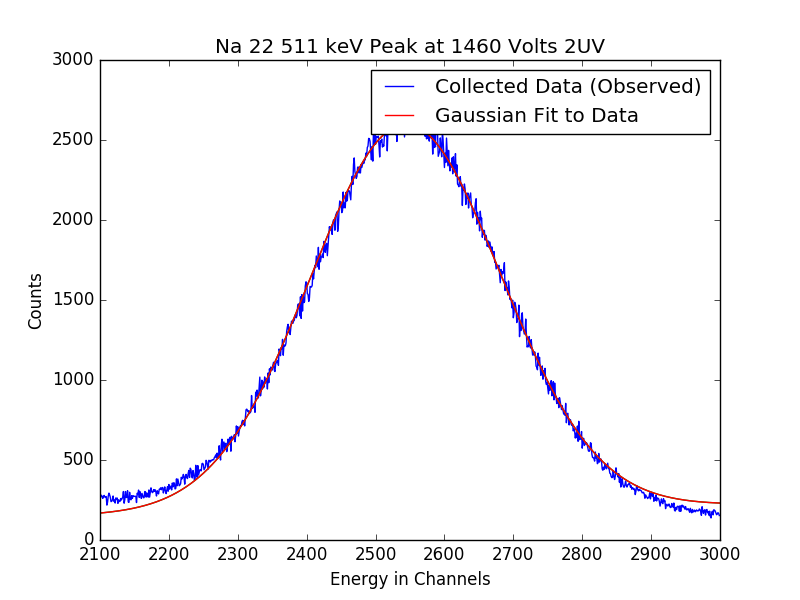
\includegraphics[width=.8\columnwidth]{2UVNa1fit.png}}%
  \qquad
  \subfloat[\label{fig:2UVNa2fit} Na 22 Peak 2 UV PMT]{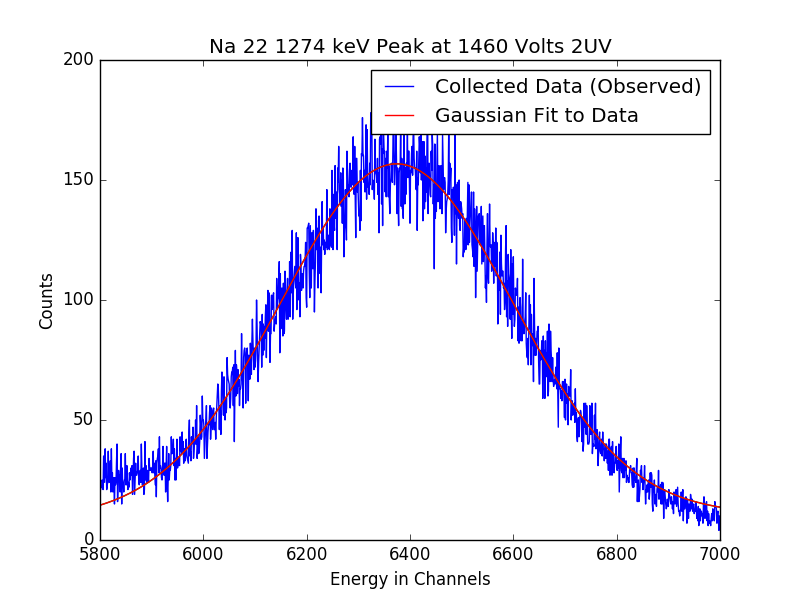
\includegraphics[width=.8\columnwidth]{2UVNa2fit.png}}%
  \qquad
  \subfloat[\label{fig:2UVRa1fit} Ra 226 First Three Peaks UV PMT]{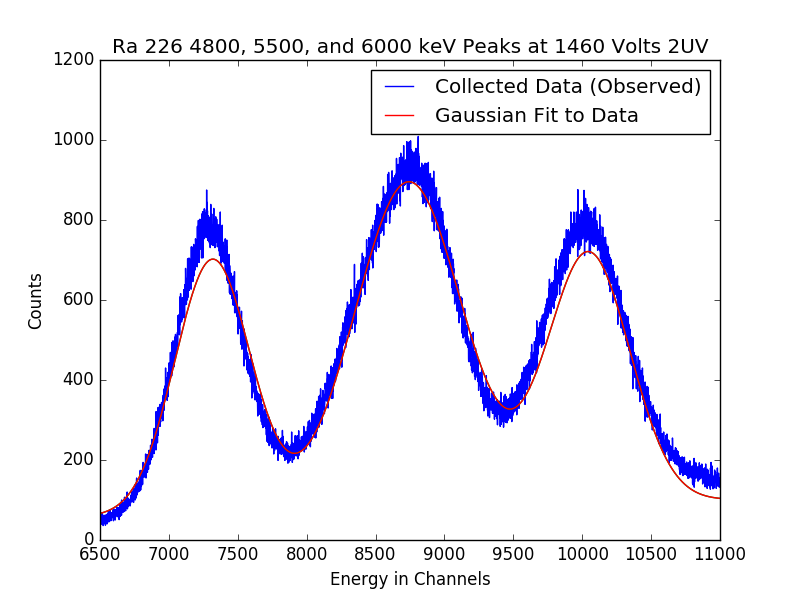
\includegraphics[width=.8\columnwidth]{2UVRa1fit.png}}%
  \qquad
  \subfloat[\label{fig:2UVRa4fit} Ra 226 Fourth Peak UV PMT]{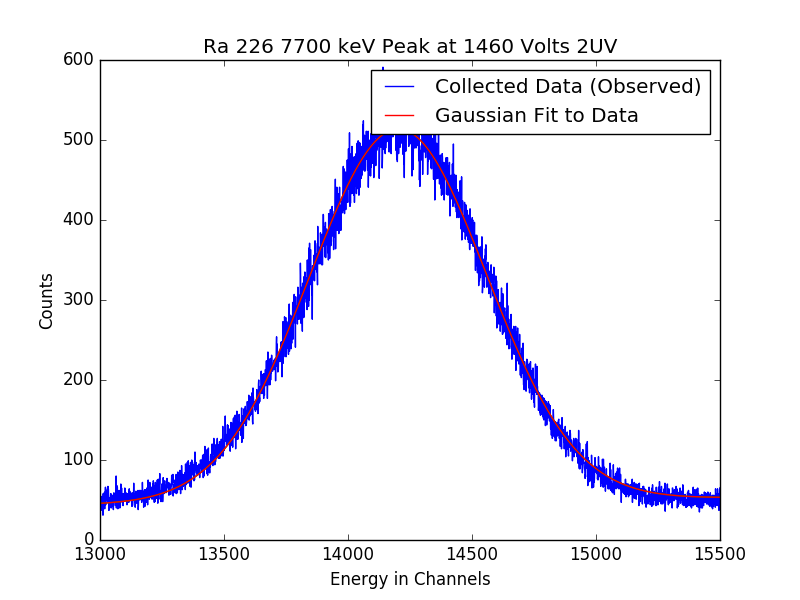
\includegraphics[width=.8\columnwidth]{2UVRa4fit.png}}%
  \qquad
\caption{All of the Gaussian fits for the Ultra-violet extended full spectrum PMT}
\end{figure*}

\begin{figure*}
  \centering
  \subfloat[\label{fig:FilCsfit} Cs 137 UV with filter PMT]{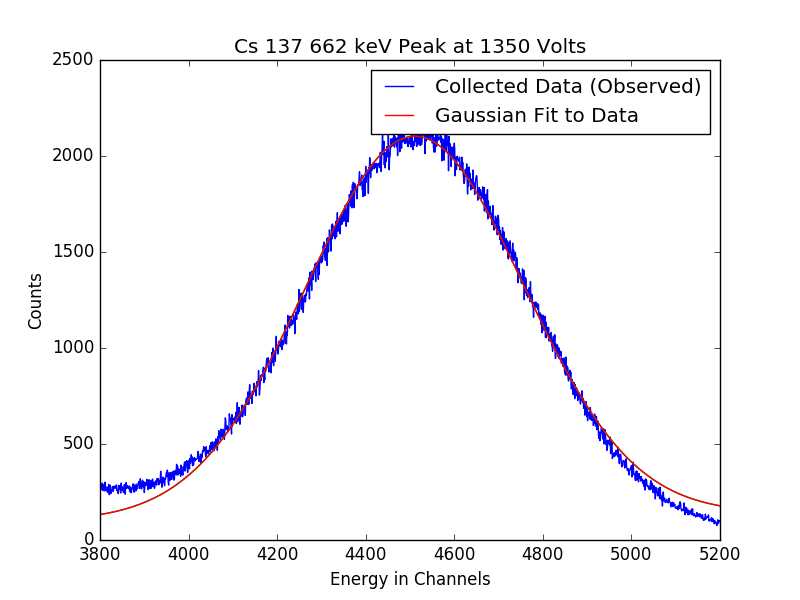
\includegraphics[width=.8\columnwidth]{FilCsfit.png}}%
  \qquad
  \subfloat[\label{fig:FilCo1fit} Co 60 Peak 1 UV with filter PMT]{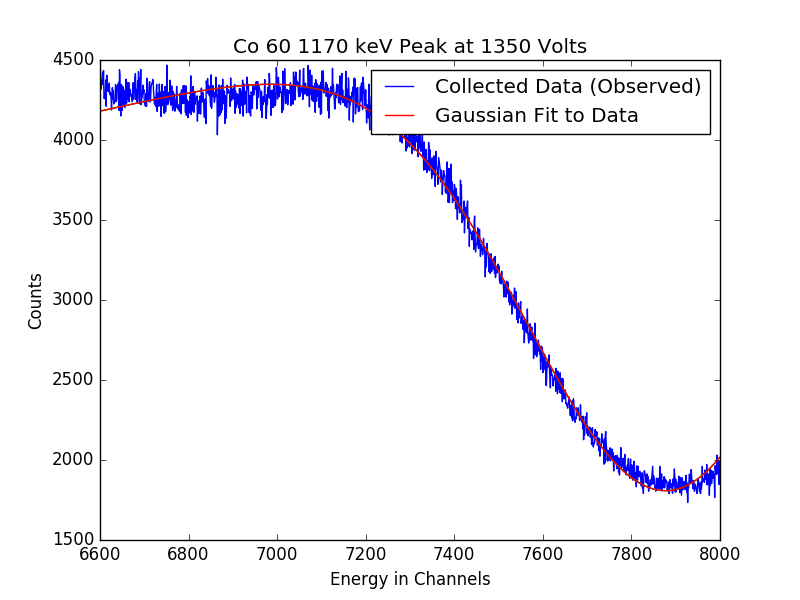
\includegraphics[width=.8\columnwidth]{FilCo1fit.png}}%
  \qquad
  \subfloat[\label{fig:FilCo2fit} Co 60 Peak 2 UV with filter PMT]{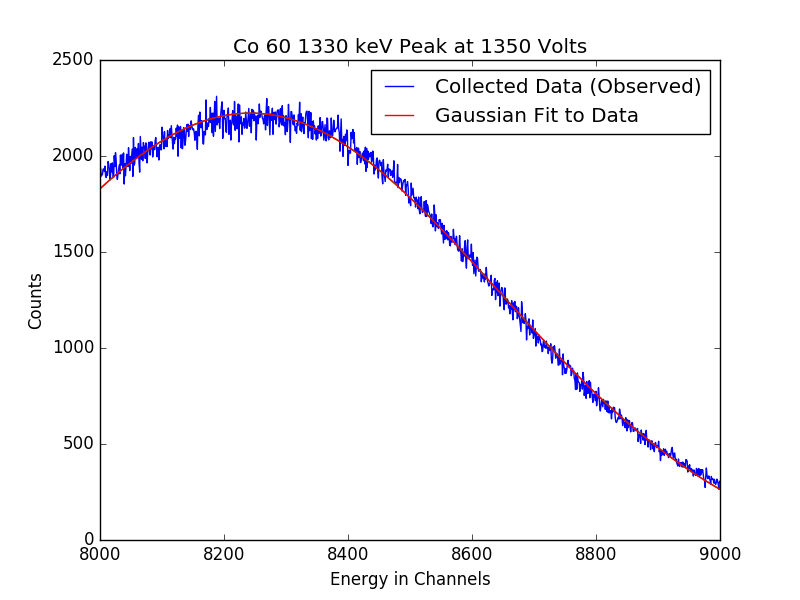
\includegraphics[width=.8\columnwidth]{FilCo2fit.png}}%
  \qquad
  \subfloat[\label{fig:FilNa1fit} Na 22 Peak 1 UV with filter PMT]{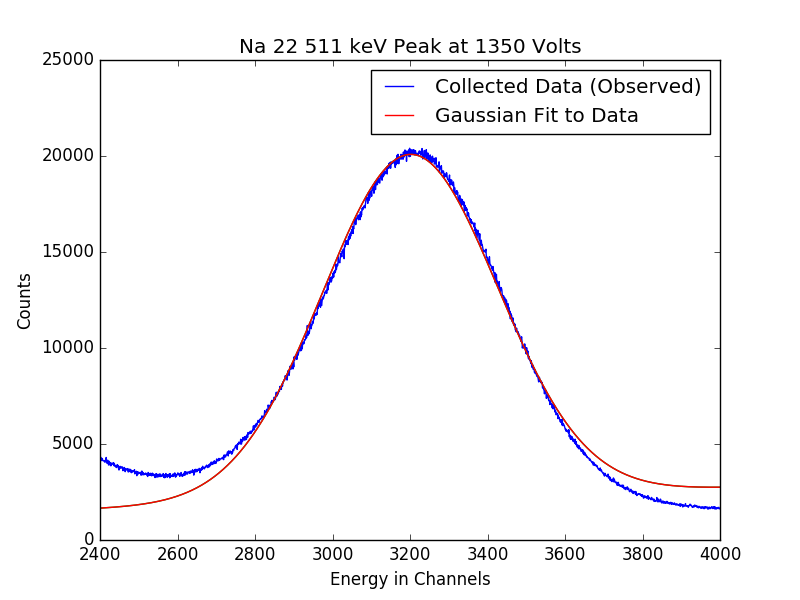
\includegraphics[width=.8\columnwidth]{FilNa1fit.png}}%
  \qquad
  \subfloat[\label{fig:FilNa2fit} Na 22 Peak 2 UV with filter PMT]{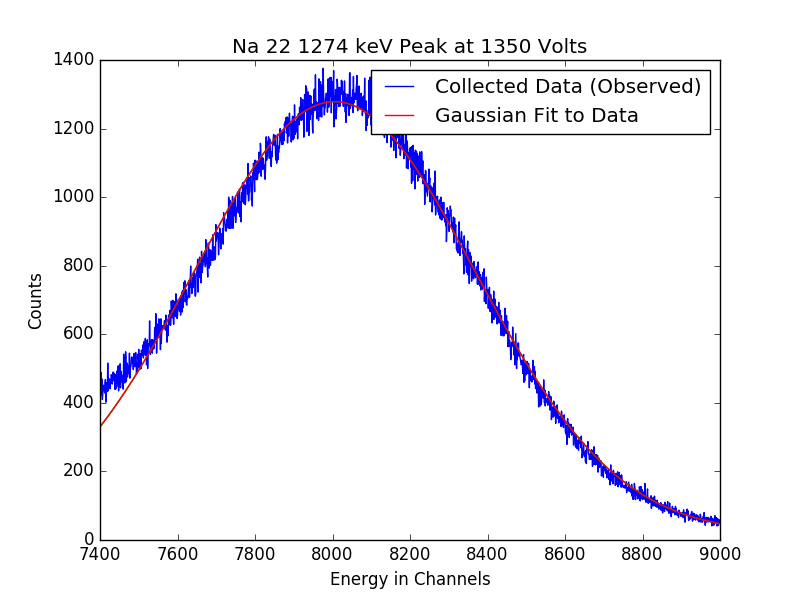
\includegraphics[width=.8\columnwidth]{FilNa2fit.png}}%
  \qquad
  \subfloat[\label{fig:FilRa1fit} Ra 226 First Three Peaks UV with filter PMT]{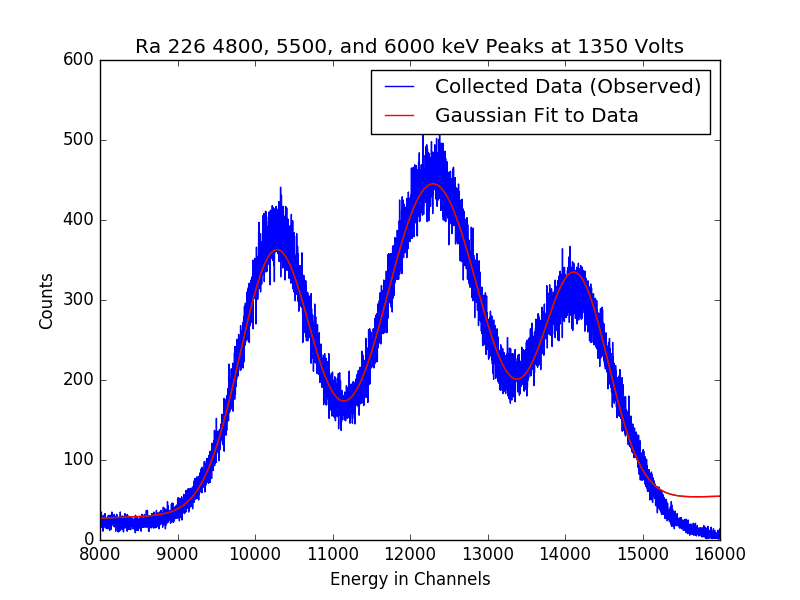
\includegraphics[width=.8\columnwidth]{FilRa1fit.png}}%
  \qquad
  \subfloat[\label{fig:FilRa4fit} Ra 226 Fourth Peak UV with filter PMT]{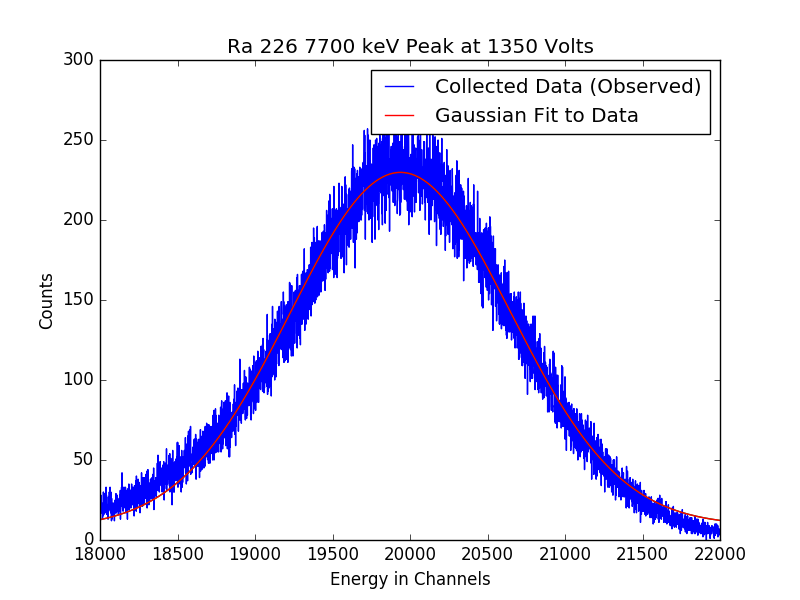
\includegraphics[width=.8\columnwidth]{FilRa4fit.png}}%
  \qquad
\caption{All of the Gaussian fits for the Ultra-violet extended sull spectrum with shortpass filter PMT}
\end{figure*}

\begin{figure*}
  \centering
  \subfloat[\label{fig:SBAmBefit} AmBe 241 Solarblind PMT]{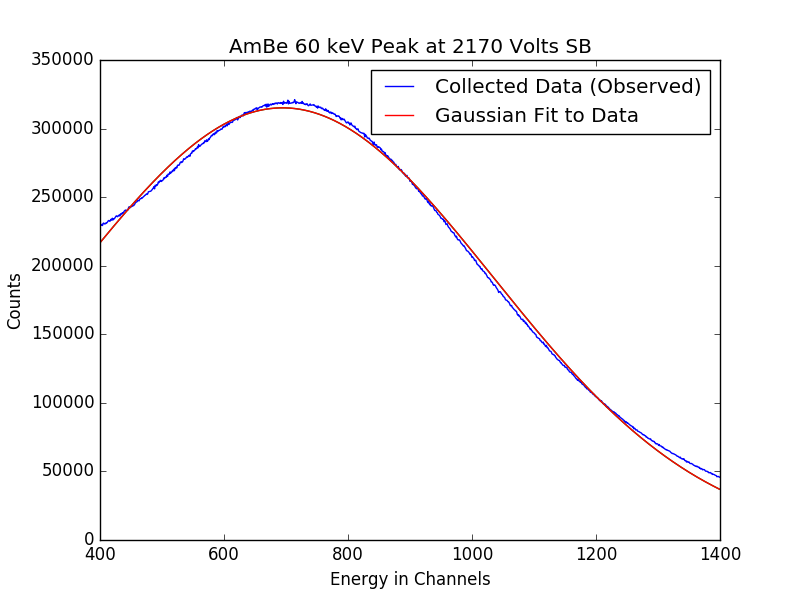
\includegraphics[width=.8\columnwidth]{SBAmBefit.png}}%
  \qquad
  \subfloat[\label{fig:SBCsfit} Cs 137 Solarblind PMT]{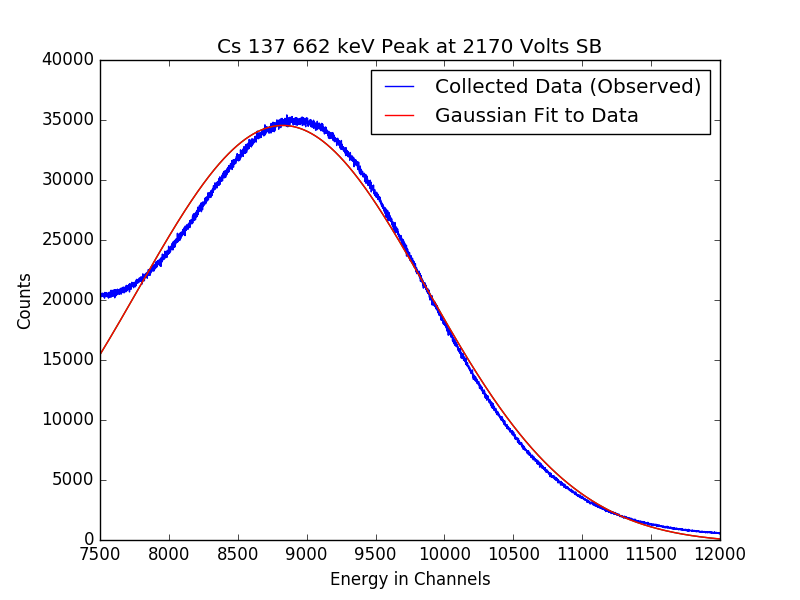
\includegraphics[width=.8\columnwidth]{SBCsfit.png}}%
  \qquad
  \subfloat[\label{fig:SBNa1fit} Na 22 Peak 1 Solarblind PMT]{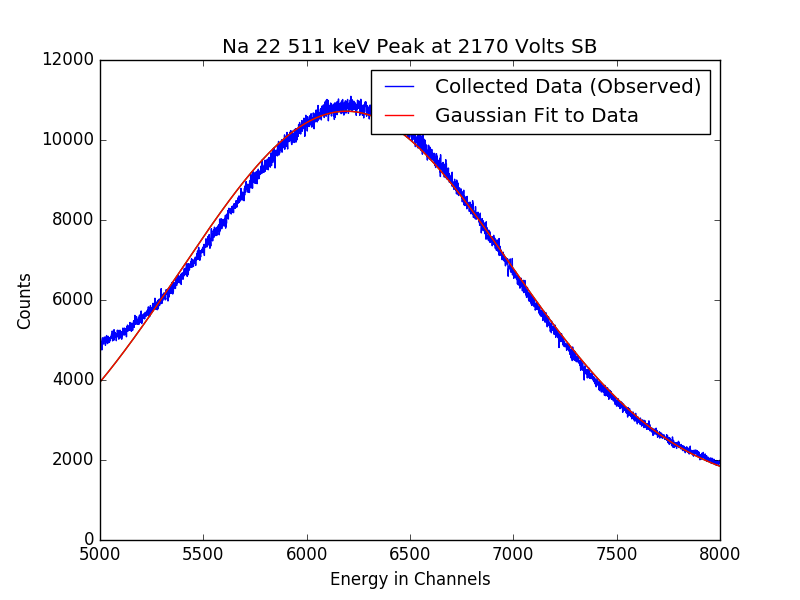
\includegraphics[width=.8\columnwidth]{SBNa1fit.png}}%
  \qquad
  \subfloat[\label{fig:SBNa2fit} Na 22 Peak 2 Solarblind PMT]{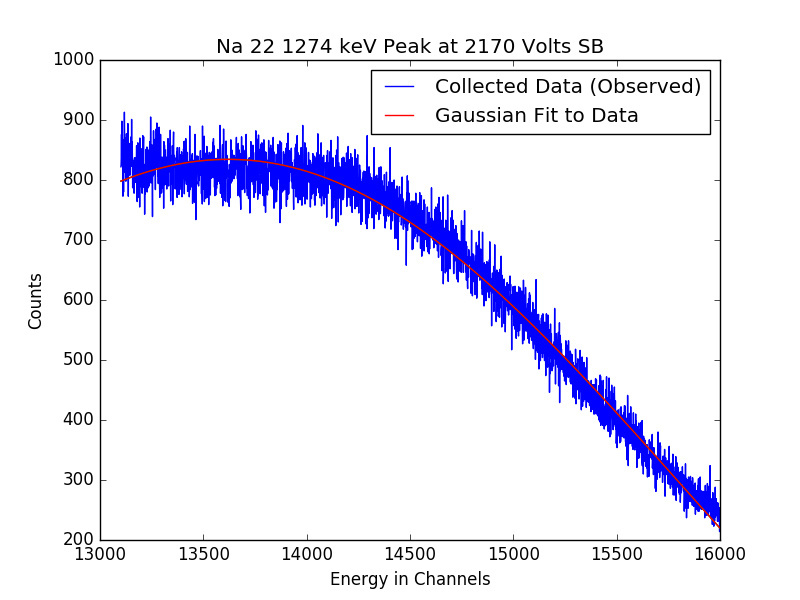
\includegraphics[width=.8\columnwidth]{SBNa2fit.png}}%
  \qquad
  \subfloat[\label{fig:SBRa1fit} Ra 226 First Three Peaks Solarblind PMT]{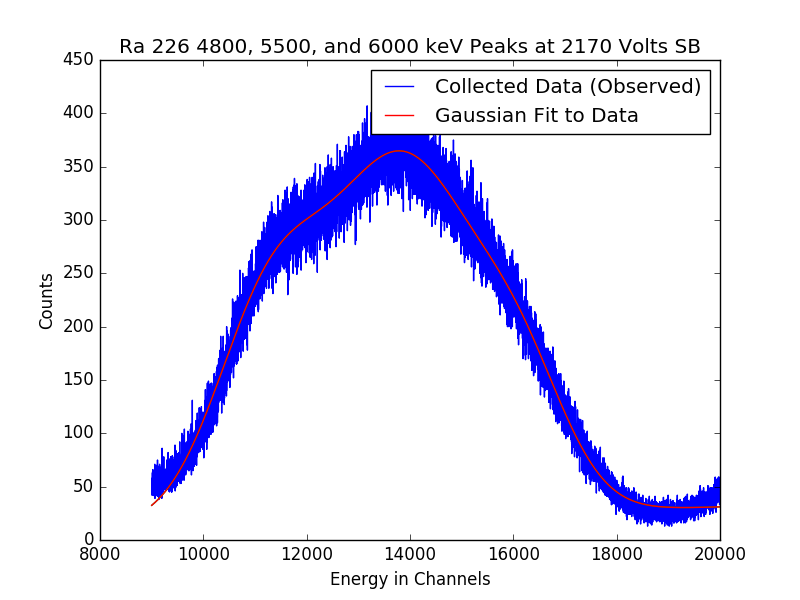
\includegraphics[width=.8\columnwidth]{SBRa1fit.png}}%
  \qquad
  \subfloat[\label{fig:SBRa4fit} Ra 226 Fourth Peak Solarblind PMT]{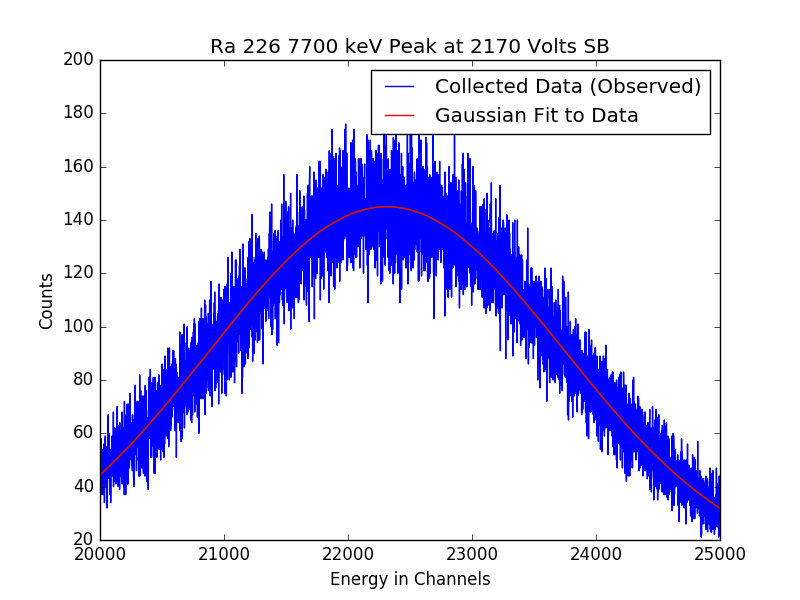
\includegraphics[width=.8\columnwidth]{SBRa4fit.png}}%
  \qquad
\caption{All of the Gaussian fits for the Solarblind PMT}
\end{figure*}

\begin{figure*}
  \centering
  \subfloat[\label{fig:UVQE} UV Quantum Efficiency]{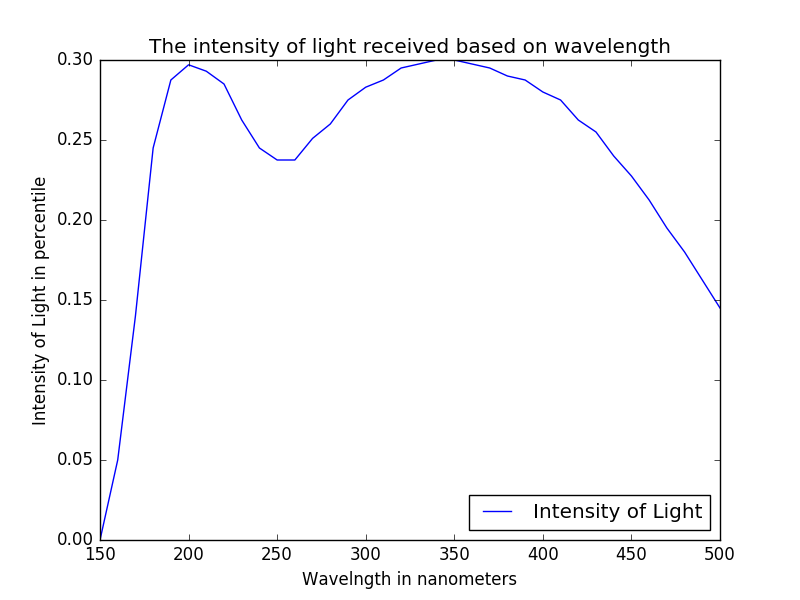
\includegraphics[width=.8\columnwidth]{UVQE.png}}%
  \qquad
  \subfloat[\label{fig:FilQE} UV with filter Quantum Efficiency]{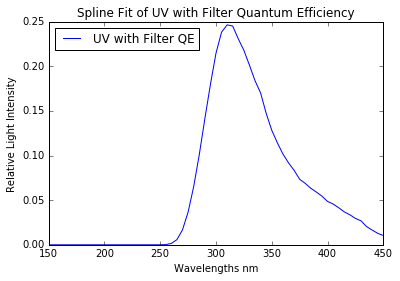
\includegraphics[width=.8\columnwidth]{FilQE.png}}%
  \qquad
  \subfloat[\label{fig:SBQE} Solarblind Quantum Efficiency]{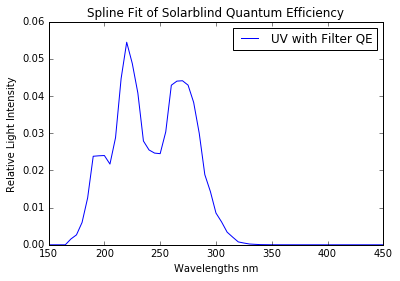
\includegraphics[width=.8\columnwidth]{SBQE.png}}%
  \qquad
\caption{All of the Quantum Efficiency Plots for each PMT}
\end{figure*}

\end{document} 




